\chapter{Imagerie de flux 4D du système cardiovasculaire de la souris rehaussée par des nanoparticules de fer avec une séquence UTE.}
\setlength{\footskip}{50pt}
\chaptermark{Imagerie 4D de mesure de flux}
\label{Chap6}
\section{Contexte}

L'accès à des paramètres fonctionnels de manière non invasive est un des enjeux des méthodes d'imagerie moderne. Leur intérêt en terme de diagnotic et de pronostic a déjà été démontré au travers de nombreuses applications dans le domaine cardiovasculaire chez l'homme. Dans cette thèse, l'intérêt d'une méthode de mesure de flux pour la caractérisation qualitative d'un modèle préclinique de pathologie vasculaire a également été montré ici.

Parmi les méthodes quantitatives de mesure de flux, l'imagerie de phase 4D (3D + t), "4D Flow MRI" est la plus prometteuse et est actuellement la plus répandue en clinique. Son champ d'applications s'élargit d'année en année avec l'étude de pathologies cérébrales \cite{meckel2008vivo,hope2010evaluation}, rénales \cite{franccois2011renal}, hépatiques \cite{stankovic2010mr}, cardiaques \cite{geiger20114d,markl2011time} ...

Cette méthode est particulièrement intéressante car elle permet à partir d'une même acquisition d'obtenir tout au long du cycle cardiaque : des images en magnitude pour visualiser des modifications anatomiques  \cite{Eriksson:2013aa}, des images de contraste de phase pour visualiser les flux anormaux \cite{Velikina:2010hc}, des cartes de vitesse des flux \cite{Garcia:2014aa} qui peuvent ensuite être utilisées pour calculer d'autres paramètres hémodynamiques comme la différence de pression \cite{Tyszka:2000aa,bock2011vivo} ou les contraintes de cisaillement sur les parois des vaisseaux (Wall Shear Stress : WSS)\cite{Zhao:2009ng}. Cette méthode apparaît donc comme un important outil diagnostique en médecine mais son utilisation en routine clinique reste encore aujourd'hui fortement limitée en particulier à cause des temps d'acquisition requis importants (10 à 20 minutes sur un coeur entier \cite{Markl:2012pi}).

Les problématiques liées à l'utilisation de cette méthode sont exacerbées dans le cas de l'imagerie préclinique et en particulier chez la souris. En effet, le faible rapport signal-sur-bruit ainsi que le nombre réduit de canaux des antennes à disposition sur les systèmes d'imagerie précliniques limitent l'utilisation de méthodes d'accélération parallèle. Le temps d'acquisition d'une image de flux 4D devient ainsi prohibitif. De plus, la présence de flux important (supérieur à 1 $m.s^{-1}$) dans des vaisseaux de petites tailles et avec une anatomie complexe a pour effet de favoriser le déphasage intravoxel des spins et donc l'apparition d'artefacts de perte de signal sur les images. Pour réduire ces artefacts, la méthode la plus simple est de réduire le temps d'écho \cite{staahlberg1994pulse,OBrien:2008aa}. L'amélioration des systèmes de gradients que ce soit en terme d'intensité ou de temps de montée, a permis d'atteindre des valeurs de temps d'écho inférieures à 2 ms en imagerie cartésienne conventionnelle. Néanmoins, ces séquences restent inférieures en terme de qualité d'images (artefacts de mouvement et de flux) que les séquences d'imagerie radiale.

Nous avons montré dans le chapitre précédent qu’en combinant des séquences à temps d’écho ultra-court (UTE) à une injection d’agent de contraste de type USPIO, il est possible de générer des images avec un très fort rapport signal-sur-bruit pour le sang et un très bon contraste-sur-bruit entre le sang et le myocarde, tout ceci sans artefact de flux ni de mouvement. De plus, ces nanoparticules possèdent une forte rémanence vasculaire, ce qui permet de conserver de forts SSB et CSB pendant au moins 1 heure.

C’est donc logiquement, que la séquence à TE ultracourt a été adaptée pour la mesure de flux par imagerie de phase 4D chez la souris. Pour cela, des gradients bipolaires ont été insérés entre l’impulsion radio-fréquence non selective et la lecture du signal. Un schéma d’encodage original a été proposé afin de permettre un meilleur moyennage des vitesses en fonction de l’instant du cycle cardiaque. 
Cette séquence a évidemment été couplée a l’injection de nanoparticules de fer afin de rehausser le rapport signal-sur-bruit du sang. En effet, le bruit sur les cartes de vitesse des flux est inversement proportionnel au signal sur les images en magnitude.

La méthode développée a d’abord été validée sur fantôme. Les mesures de vitesse effectuées ont été comparées à celles mesurées avec une séquence cartésienne sur un fantôme de flux. L’impact de la réduction des valeurs $T_2^*$ dans le cas de l’utilisation de nanoparticules de fer sur la mesure des vitesses sera évalué. Cette méthode a ensuite été utilisée sur un modèle de souris afin d’évaluer les vitesses de flux à chaque instant du cycle cardiaque sur l’entièreté du système cardio-pulmonaire de l’animal. Des résultats préliminaires ont été obtenus en comparant deux populations de souris, la première exposée à des conditions hypoxiques pendant 3 semaines et l’autre en conditions normales.

%L'utilisation de trajectoires non-cartésiennes permet d'atteindre des temps d'écho encore plus réduits ainsi que de limiter la sensibilité aux artefacts de flux. O'Brien et al  \cite{OBrien:2009ul} ont montré que l'utilisation d'une séquence 2D de mesure de flux basée sur une trajectoire radiale UTE permettait en réduisant le TE à 0.6 ms, d'obtenir des mesures plus précises grâce à la réduction des artefacts de déphasage des spins dans le cas des flux ayant une vitesse rapide.  Janiczek et al \cite{Janiczek:2011qm} ont développé et appliqué une séquence 3D de mesure de flux de type empilement de spiral sur la crosse aortique d'une souris et qui, grâce à l'effet temps-de-vol, permet d'obtenir un rapport signal-sur-bruit suffisant pour dériver le WSS. Ils ont montrés dans cette étude que cette trajectoire permet d'obtenir un meilleur signal-sur-bruit que la séquence cartésienne et est moins sensible aux artefacts de flux dans les régions présentant des vitesses rapides et incurvées. Récemment Kadbi et al \cite{Kadbi:2014uq} ont étudié l'utilisation d'une séquence 3D Stack-Of-Star UTE pour la quantification des flux sténotiques et ont montré que cette stratégie permet d'obtenir des résultats en accord avec les mesures cartésiennes pour les flux lents mais surtout de meilleurs résultats dans les cas des flux rapides.

\section{Stratégie de mesure de flux 4D}

\subsection{Introduction à la mesure de flux par imagerie de phase}

\subsubsection{Encodage de vitesse}

La quantification des flux grâce à la phase en IRM utilise l'ajout d'un gradient bipolaire entre l'excitation radiofréquence et la lecture du signal. La figure \ref{fig:PhaseSpins} montre l'effet du gradient bipolaire d'encodage de vitesse sur des spins fixes et mobiles et en particulier l'accumulation de la phase. On observe qu'à la fin du gradient bipolaire la phase des spins fixes retourne à sa position initiale alors que celles des spins mobiles accumulent une différence par rapport à l'état initial qui est directement proportionnelle à leur vitesse.

\begin{figure}[H]
\centering
\line(1,0){400} \\
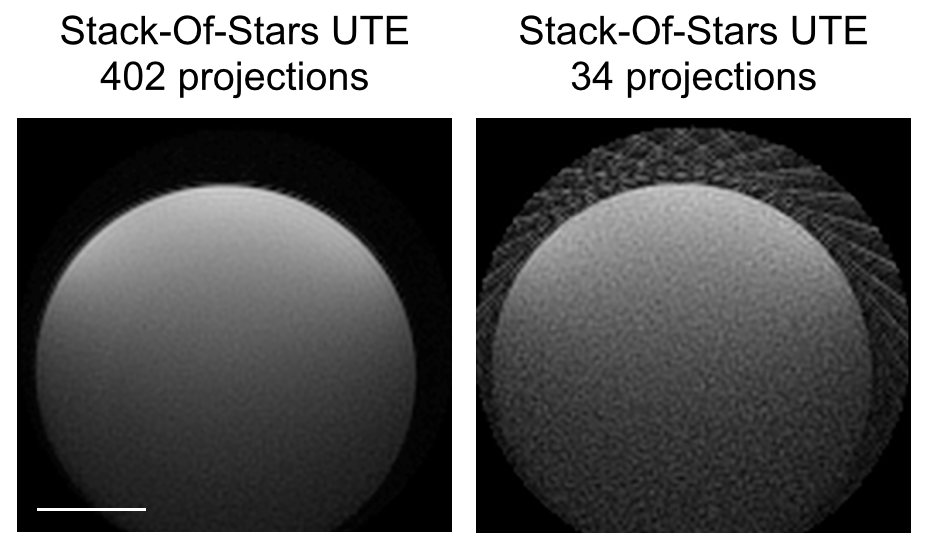
\includegraphics[scale=0.5]{./figure/chap6/Fig1.png}
\caption[Effet du gradient bipolaire sur des spins fixes et mobiles.]{\label{fig:PhaseSpins} \textbf{Effet du gradient bipolaire sur des spins fixes et mobiles.} Représentation schématique de l'évolution de la phase au cours du temps dans le cas de spins fixes et de spins mobiles sous l'influence d'un gradient bipolaire. L'accumulation de phase des spins mobiles est proportionnelle à leurs vitesses. $T_l$ représente la durée d'un lobe et T l'intervalle de temps entre le départ des deux lobes. }
\line(1,0){400} \\ 
\end{figure}
Si l'on définit la position des spins en fonction du temps de la manière suivante :
\begin{align}
x(t)=x_0 + v_0 t +a_0 t^2 + ... + \frac{1}{n!} \left(\frac{d^n x}{dt^n}\right)_{t=0} t^n
\end{align}
%x(t)=x(0) + x_1 t +\frac{1}{2!} x_2 t^2 + ... + \frac{1}{n!} x_n t^n
où $x_0$, $v_0$ et $a_0$ représente respectivement la position, la vitesse et l'accélération initiale au temps $t=0$ selon la direction du gradient bipolaire. Alors l'accumulation de phase après l'application du gradient bipolaire peut se calculer grâce à l'équation suivante :

\begin{align}
\phi (T) &= \gamma \int_0^T G(t) x(t) dt \\
			 &= \gamma (m_0(T) x_0 + m_1(T) v_0 + \frac{1}{2} m_2(T) a_0 ...)
\end{align}
où m représente le moment du gradient et le $n^{\text{ième}}$ moment de gradient m est défini par :
\begin{align}
m_n (T) &= \int_0^T G(t) t^n dt			
\end{align}
Le moment du gradient $m_0$ donne des informations sur la position des spins, $m_1$ sur la vitesse, $m_2$ sur l'accélération, etc.
Dans notre cas, on désire mesurer la vitesse des flux, il est donc nécessaire que le moment de gradient $m_0$ soit nul. C'est-à-dire que l'aire globale du gradient bipolaire soit égale à 0 (ce qui est le cas dans la figure \ref{fig:PhaseSpins}). Le moment $m_1$ représenté dans cette figure peut être calculé directement :
	
	\begin{equation}
	\begin{split}
	m_1 &= \int_{t=0}^{T_L} -G \ t \ dt  + \int_{t=T}^{T+T_L} -G \ t \ dt  \\
			&= \frac{G}{2}\left(-T_L^2+(T+T_L)^2-T^2\right) \\
			&=G \ T_L \ T \\
			& = A \ T
	\end{split} 
	\end{equation}	
où $T_L$ correspond à la durée d'un lobe, T à ll'intervalle de temps entre le départ des deux lobes et A à l'aire d'un lobe (grisé sur la figure \ref{fig:PhaseSpins}). Ce résultat est ici démontré à partir d'un gradient rectangulaire, mais il est généralisable à n'importe quelle forme de gradient bipolaire en les décomposant en une infinité de rectangle de largeur infinitésimale. Ce résultat s'applique donc aussi aux gradients avec une forme trapézoïdale qui est la forme de gradient la plus couramment utilisée dans les séquences.

L'accumulation de phase $\Phi$ pour un groupe de spins ayant une vitesse constante $v$ est donc égale à :
\begin{equation}
\label{eq:VitessePhase}
\Phi = \gamma A \ T \ v
\end{equation}
Ainsi, en modifiant la valeur de l'intensité du gradient bipolaire ou sa durée d'application, il est donc possible de modifier l'écart de phase résultant des spins mobiles en fonction de leurs vitesses.

\subsubsection{Quantification de la vitesse par imagerie de phase}

Pour mesurer la vitesse des spins, il est nécessaire de supprimer la phase statique des tissus produite par les hétérogénéités du champ magnétique $B_0$. La méthode généralement employée consiste à acquérir deux images de phase avec des intensités de gradient bipolaire différentes et ensuite de les soustraire.

Les deux méthodes les plus employées sont représentées dans la figure \ref{fig:MethodeGradientBip}.a et b. 
La méthode (a) est la méthode initialement proposée. Elle consiste à réaliser une image de phase avec un gradient bipolaire et à soustraire cette image à une autre image obtenue sans gradient bipolaire. Elle est encore souvent utilisée car l’image sans gradient bipolaire est moins sensible aux artefacts de déphasage dû au flux et peut être employée comme image de référence en magnitude.
La méthode (b) consiste à utiliser des gradients d’intensités opposées pour l’acquisition de chacune des images. Elle permet de diviser d’un facteur 2 l’intensité maximum des gradients d’encodage des vitesses par rapport à la méthode (a).
C'est cette méthode (b) décrite dans la figure \ref{fig:MethodeGradientBip}.b qui a été employée pour générer les images montrées dans la figure  la figure \ref{fig:MethodeGradientBip}.c. De l’eau circule dans un fantôme de flux (de bas en haut pour le tube de gauche et de haut en bas pour le tube de droite). Après soustraction des deux images acquises, la valeur de la phase apparaît homogène dans les deux tubes et avec une valeur opposée. A partir de cette image, la vitesse du flux peut être précisément mesurée à l'aide de l'équation \ref{eq:VitessePhase}. On trouve pour le tube de gauche une vitesse de : $v=0,2679 \pm 0,0063$ $m.s^{-1}$ et pour le tube de droite : $v=0,2478 \pm 0,0104$ $m.s^{-1}$.

\begin{figure}[h]
\centering
\line(1,0){400} \\
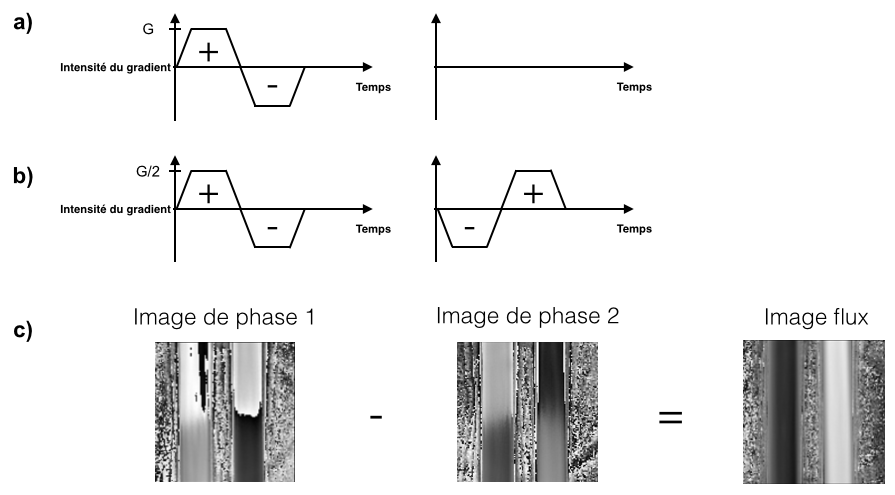
\includegraphics[scale=0.5]{./figure/chap6/Fig2.png}
\caption[Représentation de deux méthodes d'encodage de vitesse gradient bipolaire]{\label{fig:MethodeGradientBip} \textbf{Représentation de deux méthodes d'encodage des vitesses.} La méthode \textbf{(a)} consiste à recueillir une première image avec une intensité G et l'autre avec une intensité des gradients nulle. La méthode\textbf{(b)} consiste à inverser la polarisation des gradients bipolaires entre les deux images dont l'intensité utilisée est deux fois moindre que pour la méthode (a). Les deux méthodes permettent d'obtenir la même amplitude de codage des vitesses définies par $\Delta m_1 = m_1(image1) - m_1(image2)$. \textbf{(c)} La soustraction des deux images de phase permet d'obtenir une image de mesure de flux. }
\line(1,0){400} \\ 
\end{figure}

\subsubsection{Vitesse d'encodage}

Lorsque la vitesse des spins est trop importante, il est possible que leurs phases $| \Phi | > \pi$, on observe alors un repliement de la phase qui est problématique pour déterminer la vitesse des spins. Le paramètre de vitesse d'encodage des spins souvent noté VENC pour "Velocity ENCoding" a donc été inventé et est généralement exprimé en c$m.s^{-1}$. Celui-ci est fixé par l'utilisateur et correspond à la vitesse maximum qui peut être encodée sans observer de repliement de la phase. Il est donc défini à partir du moment $\Delta m_1=m_1(image_1)-m_1(image_2)$ :
\begin{align}
\text{VENC} = \frac{\pi}{\gamma | \Delta m_1 |}
\end{align} 

En réalité, l'utilisateur va définir le paramètre VENC qui permettra alors de calculer l'intensité/durée des gradients bipolaires permettant d'obtenir un encodage des vitesses correspondant à cette valeur. Dans le cas des gradients trapézoïdaux présentés dans la figure \ref{fig:MethodeGradientBip} qui sont ceux implémentés dans cette séquence, l'intensité des gradients d'encodage G est définie par :

\begin{align}
G = \frac{\pi}{2 \gamma \ T_L \ T \ \text{VENC}}
\end{align}
En posant r le temps de montée et de descente des gradients et d la durée du plateau des gradients trapezoïdaux de la figure \ref{fig:MethodeGradientBip}, on obtient alors $T_L = d+r$ et $T = d+2r$.

La valeur de VENC choisi par l'utilisateur doit être supérieure à la vitesse maximum supposée pour éviter tout repliement. Mais elle doit aussi aussi être relativement assez proche des vitesses à observer car le paramètre de vitesse-sur-bruit (VSB) dans les cartes de vitesse (l'équivalent du signal-sur-bruit (SSB)) suit la loi suivante :
\begin{align}
\text{VSB} \propto \frac{V}{\text{VENC}}\text{SSB}
\end{align}
 Généralement le paramètre VENC est choisi de manière à être 30$\%$ supérieur à la vitesse maximum qui peut être observer \textit{in vivo}. 

\subsubsection{Antennes multicanaux et reconstruction des images de mesure des flux}

Pour reconstruire une image réalisée avec une antenne multicanaux, la méthode couramment utilisée consiste à combiner les images en magnitude obtenues avec chacun des canaux par la méthode de racine carrée de somme des carrées. Néanmoins, avec cette stratégie l’information de phase dans l’image finale est perdue.
Deux méthodes peuvent être utilisées pour obtenir des images de phase à partir de l’antenne à 4 canaux que nous avons utilisée.

Soit $I_1$ et $I_2$, des images complexes qui sont acquises avec l'une des stratégies de contraste de phase définies dans la partie précédente. Ces images peuvent être représentées en utilisant leur magnitude (A) et phase ($\Phi$) respectives :
\begin{equation}
\begin{split}
I_1= A_1 . e^{i \Phi_1} \\
I_2= A_2 . e^{i \Phi_2}
\end{split}
\end{equation}
La carte de contraste de phase $\Delta \Phi$ pour une antenne à un élément peut alors se calculer de la manière suivante :
\begin{equation}
\begin{split}
\Delta \Phi &= arg(I_1 \cdot I_2^*) \\
				  &= arg(A_1 \cdot A_2 \cdot e^{i(\Phi_1 - \Phi_2)}) \\
				  &= \Phi_1-\Phi_2
\end{split}
\end{equation}

Cette équation peut être étendue à des données recueillies avec une antenne multicanaux où l'opération de différence de phase est effectuée après la combinaison de tout les canaux individuellement.

\begin{equation}
\begin{split}
\Phi_1 &= arg( \sum_1^n  A_{1,n} \cdot e^{i \Phi_{1,n}}) \\
\Phi_2 &= arg( \sum_1^n  A_{2,n} \cdot e^{i \Phi_{2,n}}) \\
\Delta \Phi &= \Phi_1 - \Phi_2
\end{split}
\end{equation}

Une autre méthode disponible décrite par Bernstein et al \cite{bernstein1994reconstructions} consiste à effectuer l'opération de différence de phase individuellement pour chaque canal puis d'additionner les données avant de générer la carte de phase :

\begin{align}
\Delta \Phi = arg(\sum_1^n A_{1,n} \cdot A_{2,n} \cdot e^{i(\Phi_{1,n} - \Phi_{2,n})})
\end{align}

Dans ce chapitre, la méthode employée est la méthode de Bernstein qui s'avère donner de meilleurs résultats.

\subsection{Chronogramme de la séquence 4D UTE de contraste de phase}

\begin{figure}[H]
\centering
\line(1,0){400} \\
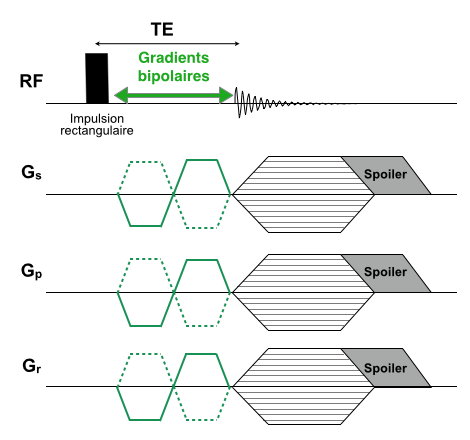
\includegraphics[scale=0.5]{./figure/chap6/Fig3.png}
\caption[Chronogramme de la séquence 4D UTE de contraste de phase.]{\label{fig:Chrono4DFlux}\textbf{ Chronogramme de la séquence 4D UTE de contraste de phase.} Des gradients bipolaires (en vert) sont présents entre l'excitation radiofréquence non-sélective et la lecture du signal. La polarité et l'intensité des gradients bipolaires est définies en fonction de la méthode d'encodage des vitesses employée.}
\line(1,0){400} \\ 
\end{figure}

Afin d’encoder les vitesses dans les 3 directions de l’espace et en fonction du rythme cardiaque, une nouvelle séquence d’imagerie de flux a été développée.

Cette séquence décrite dans la figure (\ref{fig:Chrono4DFlux}) est basée sur la séquence 3D UTE présentée dans le chapitre \ref{Chap4}.  Des gradients bipolaires de codage de vitesses (en vert) ont été introduits entre l’impulsion radiofréquence et la lecture du signal. La lecture du signal se fait de manière radiale en partant du centre de l’espace de Fourier. La trajectoire des projections est la même que celle décrite dans le chapitre \ref{Chap4}, elle permet de positionner les derniers points de chaque projection en suivant une trajectoire spiralée sur la surface d'une sphère.

En utilisant des intensités de gradients élevées, il est possible de limiter le temps d’applications des gradients bipolaires. Dans notre cas, des valeurs de VENC de 0.6 $m.s^{-1}$ peuvent être atteintes pour une durée de gradient de 0,421 ms correspondant à des intensités de gradients de 52 $\%$ par rapport à l'intensité maximum des gradients de 660 $mT.m^{-1}$. Associé à la durée réduite de l'impulsion de radiofréquence, les valeurs de TE obtenues restent faibles entre 0.450 et 0.550 ms. Les avantages liés au temps d'écho ultra-court restent ainsi vrais pour cette séquence.

\newpage
\subsubsection{Gradients de codage de vitesse}

Les gradients bipolaires utilisés dans ce travail sont des gradients trapézoïdaux définis par leurs temps de montée \textbf{\textit{r}}, la durée du plateau \textbf{\textit{d}} et l’intensité maximum \textbf{\textit{G}}. La polarité du premier lobe peut être positive ou négative correspondant respectivement aux traits pointillés et pleins sur la figure \ref{fig:EncFlux}.

Pour mesurer la vitesse selon les 3 directions de l'espace, il est nécessaire d'encoder les vitesses selon les 3 axes. Ceci requiert au minimum 4 acquisitions avec des combinaisons de gradients bipolaires différentes. Plusieurs combinaisons de gradients bipolaires peuvent être utilisées \ref{fig:EncFlux} : 4-points standard, 4-points symétrique, 4-points Hadamard. 

\begin{figure}[H]
\centering
\line(1,0){400} \\
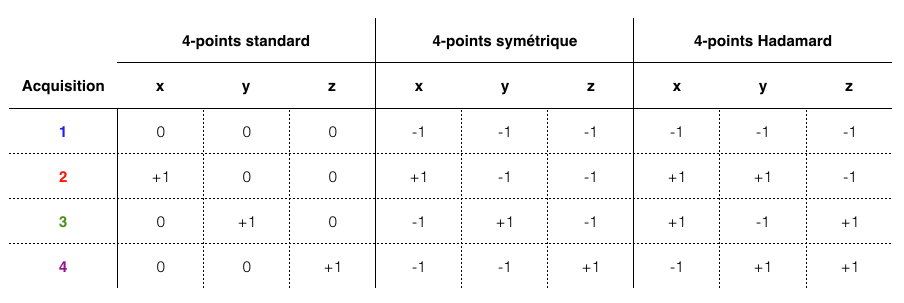
\includegraphics[scale=0.45]{./figure/chap6/Fig4.png}
\caption[Présentation de 3 méthode d'encodage de flux.]{\label{fig:EncFlux} \textbf{Tableau représentant la polarité des gradients bipolaires pour 3 méthodes} : 4-points standard, 4-points symétrique et 4-points Hadamard. Pour obtenir le même encodage des vitesses pour la méthode standard, l'intensité des gradients bipolaires est 2 fois plus importante que pour les deux autres méthodes.}
\line(1,0){400} \\ 
\end{figure}

\subsubsection{Reconstruction des cartes de vitesses}

Pour obtenir les cartes de vitesses à partir des reconstructions de chaque acquisitions, la combinaison des données est différente en fonction de la méthode de codage employée. Pour les méthodes standard et symétrique, les cartes de vitesses ($V_x,V_y,V_z$) sont obtenues en combinant les cartes de phase des acquisitions, notées $Acq_i$ (i=1, 2, 3 ou 4) selon la méthode suivante :

\begin{equation}
\begin{split}
V_x = (Acq_2-Acq_1) \frac{\text{VENC}}{\pi} \\
V_y = (Acq_3-Acq_1 ) \frac{\text{VENC}}{\pi}\\
V_z = (Acq_4-Acq_1 ) \frac{\text{VENC}}{\pi}
\end{split}
\end{equation}

Pour la méthode d’encodage Hadamard, chaque carte de vitesse ($V_x$, $V_y$, $V_z$) combine toutes les données acquises selon la méthode suivante : 

\begin{equation}
\begin{split}
V_x = (-Acq_1+Acq_2+Acq_3-Acq_4) \frac{\text{VENC}}{\pi} \\
V_y = (-Acq_1+Acq_2-Acq_3+Acq_4 ) \frac{\text{VENC}}{\pi}\\
V_z = (-Acq_1-Acq_2+Acq_3+Acq_4 ) \frac{\text{VENC}}{\pi}
\end{split}
\end{equation}

Les méthodes 4-points symétrique et Hadamard ont été testées. En effet, elles permettent de réduire l’intensité maximale des gradients d’un facteur 2 par rapport à la méthode standard pour la même valeur de VENC. Il est donc possible en utilisant 100 pourcents de l'intensité des gradients de réduire la durée des gradients de codage de vitesse et par conséquence le temps d’écho de la séquence.

Finalement, le choix définitif s'est porté sur la méthode symétrique. En effet, la plage dynamique des vitesses qui peuvent être mesurées avec la méthode Hadamard sans obtenir de repliement est dépendante de la direction de la vitesse des flux. Il est ainsi possible d'obtenir un repliement de la phase si la vitesse est supérieur à $v=\text{VENC}/\sqrt{2} $ selon 2 directions d'encodage des vitesses \cite{Pelc:1991aa} contrairement à la méthode d'encodage symétrique.

\subsection{Stratégie d'encodage 4D de vitesse des flux}

Pour mesurer les vitesses de flux en fonction du cycle cardiaque, la séquence est synchronisée prospectivement sur l’onde R de l'ECG. Au cours d'un cycle cardiaque, NCine phases sont reconstruites (Ciné 1, Ciné 2, ..., Ciné N). Chaque phase est reconstruite à partir de 4 signaux IRM permettant d'encoder la vitesse selon les 3 dimensions avec la méthode 4-points symétriques. Tous les signaux recueillis au cours du même battement de coeur ont la même trajectoire, celle-ci est définie selon la méthode présentée dans le chapitre \ref{Chap4}. Les couleurs des signaux IRM qui sont représentées sur la figure \ref{fig:SchemaAcqFlux} permettent de définir la polarité des gradients bipolaires qui sont utilisés en accord avec les couleurs des acquisitions représentées dans la figure \ref{fig:EncFlux}. 

L'ordre d'encodage des signaux IRM dans chaque phase cardiaque est déplacé d'une étape à chaque battement de coeur, puis réinitialisé après le 4$^\text{ème}$ battement. Cette stratégie permet de recueillir à chaque battement de coeur les projections permettant d'encoder les trois directions avec une même trajectoire. Le changement d'ordre d'encodage d'un battement cardiaque à l'autre permet quant à lui de moyenner le mouvement et les modifications de vitesse sur les phases cardiaques qui seront reconstruites.

\begin{figure}[H]
\centering
\line(1,0){400} \\
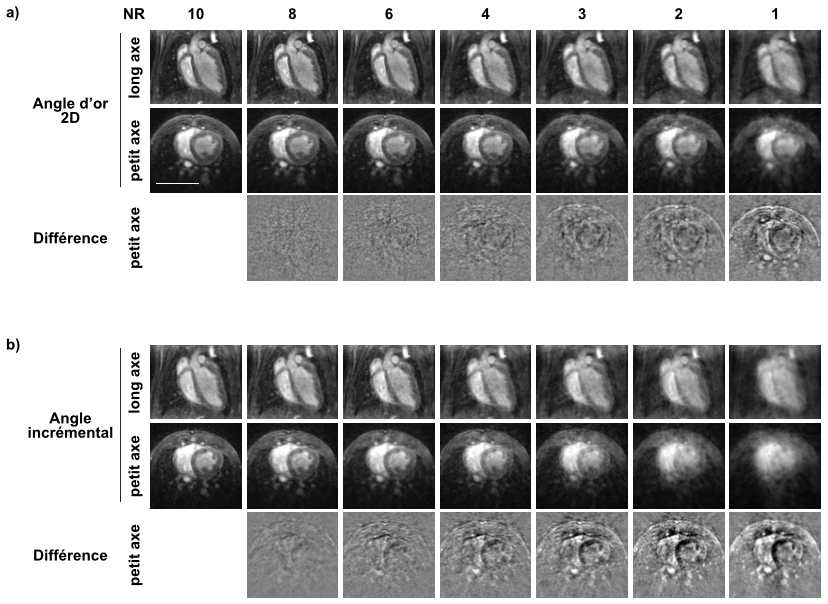
\includegraphics[scale=0.5]{./figure/chap6/Fig5.png}
\caption[Schéma acquisition des données de flux 4D.]{\label{fig:SchemaAcqFlux} \textbf{Schéma d'acquisition des données de flux 4D.} Les acquisitions sont synchronisées prospectivement sur le rythme cardiaque. Chaque couleur de FID correspondant à l'utilisation de gradient bipolaire en accord avec la figure \ref{fig:EncFlux}.}
\line(1,0){400} \\ 
\end{figure}

\subsection{Correction des erreurs de phase/vitesse}

Lors de l'acquisition des images de flux, des erreurs de phase sont souvent observées et engendrent des erreurs sur les mesures de flux. Ces erreurs proviennent principalement de 3 sources : les courants de Foucault \cite{Walker:1993aa}, les gradients concomittants \cite{Bernstein:1998aa} et les distorsions du champ de gradient provenant de la géométrie des bobines de gradient. \cite{Markl:2003aa}. 

Diverses méthodes existent pour corriger ces erreurs. Dans ce chapitre la méthode décrite par Chernobelsky et al \cite{Chernobelsky:2007aa} a été implémentée car elle permet de corriger les erreurs provoquées par les courants de Foucault et les gradients concomittants. Cette méthode consiste à appliquer la même séquence d'imagerie de flux (avec les mêmes paramètres) sur un fantôme homogène statique, puis de soustraire les cartes de vitesse obtenues avec ces données aux cartes de vitesse obtenues \textit{in vivo}. 

Un exemple d'application de cette stratégie de correction est présenté dans la figure \ref{fig:CorrectionPhase}. Sur l'image acquise non corrigée, la présence d'une erreur linéaire sur la carte de vitesse est observée (ligne pointillée). Après soustraction des images \textit{in vivo} avec l'image acquise sur le fantôme statique, l'erreur linéaire est corrigée et la vitesse apparaît uniforme tout le long du fantôme de flux (ligne pleine).

%Lorenz et al \cite{Lorenz:2014aa} ont montrés que cette stratégie permettait de grandement améliorer les résultats dans le cadre de l'utilisation de représentation des trajectoires des flux. Ils ont aussi quantifiée que l'impact des erreurs provenant des distorsions de champ de gradient était faible sur un imageur clinique. Or en imagerie préclinique le diamètre de l'aimant est plus faible ce qui réduit d'autant plus ce type d'erreur par rapport à l'étude menée par Lorenz.

\begin{figure}[H]
\centering
\line(1,0){400} \\
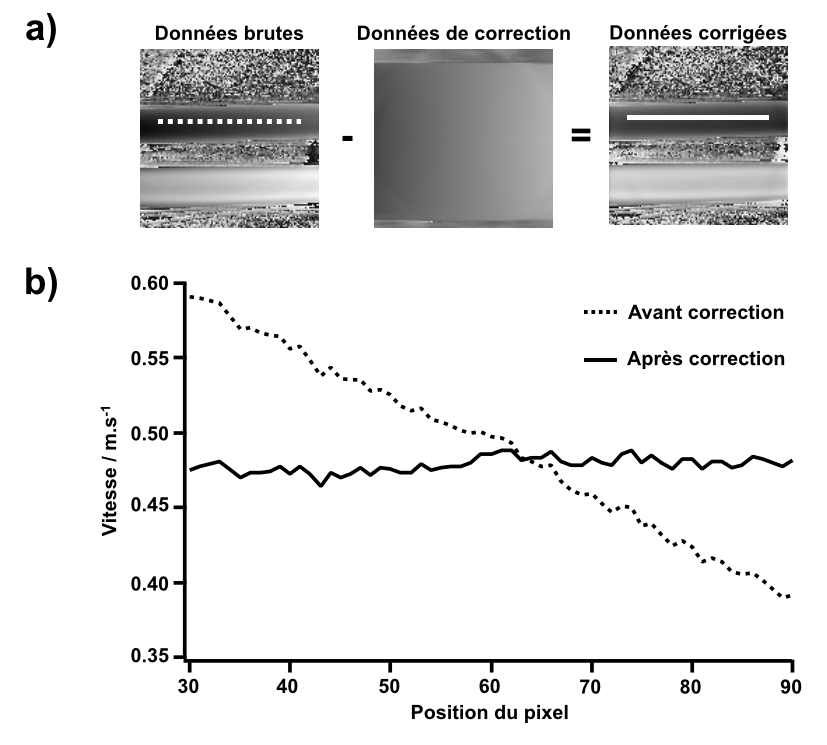
\includegraphics[scale=0.4]{./figure/chap6/Fig6.png}
\caption[Correction de la phase]{\label{fig:CorrectionPhase} \textbf{Méthode de correction des erreurs de phase.} \textbf{(a)} 
Une carte de vitesse recueillie sur un fantôme homogène est soustraite de la carte de vitesse acquises sur un fantôme de flux. L’image après correction montre l’homogénéité de la vitesse mesuré le long du tube. Le signal mesuré au niveau des lignes pointillée et pleine est représenté sur le graphique en \textbf{(b)}.}
\line(1,0){400} \\ 
\end{figure}

\section{Validation \textit{in vitro}}

La séquence a été validée sur un fantôme de flux constitué d'un tube d'eau statique et d'un tube droit effectuant un aller-retour dans le champ de vue dans lequel circule de l'eau avec du chlorure de manganèse ($\text{MnCl}_2$). Le chlorure de manganèse est utilisé à différentes concentrations allant de 0 à 8 mM ce qui permet de diminuer la valeur des $T_2$ de l'eau (de 393 à 0,8 ms) ainsi que les valeurs de $T_2*$. Il sert ainsi à mimer l'effet des nanoparticules de fer sur les temps de relaxation du sang. Le chlorure de manganèse est ici utilisé pour une question de coût.
%correspondant respectivement à un $T_2 \approx 393/6/3/1,5/1/0,8 ms$

La première étape a été de vérifier la robustesse des mesures de vitesse avec la séquence de flux 3D UTE (TE/TR = 0,571/5 ms) vis-à-vis de la diminution des valeurs de $T_2*$ qui apparaît après l'injection d'un agent de contraste à base de nanoparticules de fer. Les mêmes expériences ont été réalisées avec une séquence cartésienne FLASH (TE/TR = 2,3/5ms) de mesure de flux à titre de comparaison.
Pour cela, la vitesse dans le tube a été mesurée pour des concentrations en $\text{MnCl}_2$ de 0, 1, 2, 4, 6, 8 mM et des valeurs de VENC de 1.2, 1.0, 0.8, 0.6 $m.s^{-1}$. Le débit du flux a été fixé durant toutes les acquisitions pour générer une vitesse moyenne de 0.258 $m.s^{-1}$.

Les résultats sont présentés sur la figure \ref{fig:FluxFantT2}. Les mesures effectuées avec la séquence UTE ($v=0.267 \pm 0.0063 m.s^{-1}$) montrent une très faible dispersion que ce soit en fonction de la valeur VENC ou de la concentration en manganèse. Au contraire, les résultats obtenus avec le séquence FLASH sont beaucoup plus dispersés ($v=0.284 \pm 0.065 m.s^{-1}$). 
Néanmoins, ceci ne semble pas dû à l'effet du Manganèse sur le $T_2*$, mais s’explique plutôt par la sensibilité de la séquence cartésienne aux artefacts de flux. Ces derniers sont visibles sur les images en magnitude et s’expliquent par le caractère pulsatile de la pompe utilisée pour le fantôme de flux. La séquence UTE est quant à elle très peu sensible à ce type d’artefact et les mesures montrent donc une forte reproductibilité. 

\begin{figure}[h]
\centering
\line(1,0){400} \\
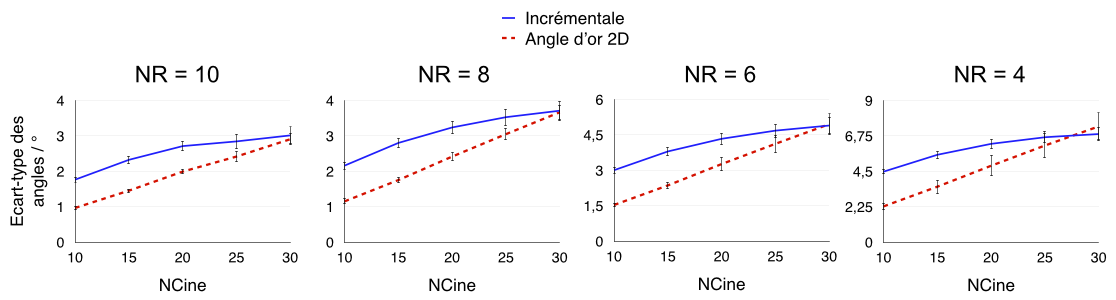
\includegraphics[scale=0.5]{./figure/chap6/Fig7.png}
\caption[Mesure du flux en fonction du $T_2*$.]{\label{fig:FluxFantT2} \textbf{Mesure des vitesse de flux en fonction du $T_2*$.} Les vitesses sont mesurées sur un fantôme de flux avec la séquence UTE 3D et une séquence cartésienne FLASH 3D en fonction de la concentration en $\text{MnCl}_2$ (0, 1, 2, 4, 6, 8 mM) et pour différentes valeurs de VENC (1.2, 1.0, 0.8, 0.6 $m.s^{-1}$). La vitesse imposée est de 0,258 $m.s^{-1}$.}
\line(1,0){400} \\ 
\end{figure}

La deuxième partie de l'étude sur fantôme a pour objectif de vérifier la linéarité des mesures de vitesse. Les mesures ont été effectuées avec les séquences FLASH cartésienne et UTE et une valeur de VENC fixée à 0,8 $m.s^{-1}$ et une concentration de $\text{MnCl}_2$ à 2 mM. Les mesures ont été répétées 3 fois pour différentes vitesses imposées dans le tube (0.497, 0.400, 0.306, 0.197 et 0.095 $m.s^{-1}$). 
Les résultats sont représentés dans la figure \ref{fig:FluxFantLinear} avec en abscisse la vitesse du flux imposée dans le tube et en ordonnée les mesures de vitesse obtenues avec les deux séquences. Les mesures de flux effectuées avec la séquence UTE montre une meilleure concordance avec le flux imposé que celle obtenues avec la séquence FLASH. De plus, les mesures montrent là encore une dispersion bien plus faible avec la séquence UTE.

La séquence UTE 3D semble donc particulièrement robuste et précise pour effectuer des mesures de flux.  Nous avons montré avec les expériences sur fantôme sa supériorité par rapport à la séquence cartésienne FLASH. De plus, l’utilisation de produit de contraste diminuant le $T_2*$ de l’eau semble avoir peu d’influence sur la reproductibilité des mesures réalisées sur fantômes.

\begin{figure}[H]
\centering
\line(1,0){400} \\
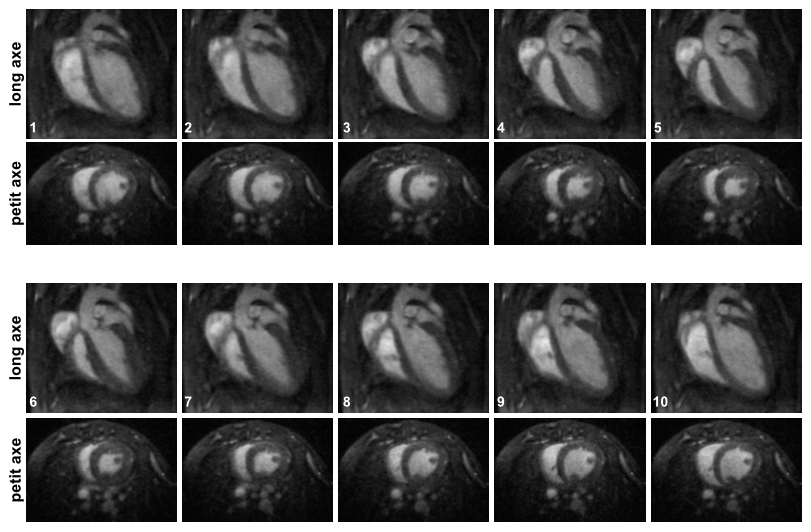
\includegraphics[scale=0.7]{./figure/chap6/Fig8.png}
\caption[Quantification des vitesses en fonction du débit imposé.]{\label{fig:FluxFantLinear} \textbf{Quantification des vitesses en fonction du débit imposé.} Mesure des vitesses sur un fantôme de flux effectuée avec la séquence UTE et une séquence cartésienne FLASH en fonction de la vitesse du flux imposée (0.497, 0.400, 0.306, 0.197, 0.095 $m.s^{-1}$). La concentration en $\text{MnCl}_2$ est de 2 mM et une valeur de VENC de 1.0 $m.s^{-1}$ est utilisée.}
\line(1,0){400} \\ 
\end{figure}


\section{Résultats préliminaires \textit{in vivo}}

Des mesures de flux ont ensuite été réalisées \textit{in vivo} sur un modèle de souris C57/Black 6.

Les expériences ont été réalisées à 7 Tesla avec une antenne de surface à 4 éléments et la séquence UTE 4D synchronisée sur le cycle cardiaque de l’animal. Les  paramètres suivants ont été employés :
TR/TE = 3.5/0.45 ms, impulsion radiofréquence rectangulaire de 0,05 ms avec une bascule de l'aimantation de 15$\degres$, champ de vue = 20 x 20 x 20, matrice = 128 x 128 x 128, résolution spatiale : 156 $\mu m$ isotropique, nombre de volumes ciné = 10, nombre de projections  = 18140, bande passante de réception = 781,25 Hz/Pixel, VENC = 1.2 $m.s^{-1}$, temps d'acquisition total $\approx$ 45 minutes.

Les souris ont été anesthésiées avec 1$\%$ d'isoflurane dans l'air. Le signal ECG est récupéré grâce à des électrodes positionnées sur la patte supérieure droite et la patte inférieure gauche. Le signal ECG recueilli est utilisé pour synchroniser l'acquisition aux battements du coeur grâce à un système de visualisation et de synchronisation spécifique (SA Instruments, Inc., NY). L'ECG est visualisé sur l'interface et le rythme cardiaque est stabilisé entre 400 et 415 battements par minute en modifiant le pourcentage d'isoflurane inhalé. 100 $\mu L$ de Sinerem sont injectés par la veine caudale de la souris à une concentration de 200 $\mu mol$ Fe/kg.

\subsection{Validation de la séquence}

Des images anatomique et de flux, obtenues chez une souris saine, sont montrées en vue coronale sur la figure \ref{fig:CarteVitesse}. Cinq des dix images réalisées pendant le cycle cardiaque sont représentées d'abord en magnitude, puis en Vx, Vy ou Vz, respectivement les composantes de la vitesse du flux selon les axes x, y ou z, et enfin en vitesse absolue. Les images en magnitude sont reconstruites à partir des données d'une seule direction d'encodage de vitesse.

Comme montré sur les images en magnitude, la combinaison de l’injection de l’agent de contraste à base de nanoparticules de fer et l’utilisation d’une séquence à temps d’écho court permet d’obtenir un rapport signal-sur-bruit élevé pour le sang (35,5 $\pm$ 2,3). De plus, aucun artefact de flux, ou de disparition de signal dû aux déphasages des spins mobiles n’est observé au cours du cycle cardiaque, que ce soit au niveau de la crosse aortique ou même de zones extrêmement turbulentes comme la cavité cardiaque.

Ainsi, grâce à cette homogénéité de signal, il est possible d’obtenir une information de phase, donc de vitesse sur l’entièreté des vaisseaux du système cardio-pulomnaire de l’animal et quel que soit l’instant du cycle cardiaque. La méthode développée permet par exemple d’apprécier la vitesse maximum élevée du sang comme dans la crosse aortique  pendant la systole  ($v_{max}$ = 0,75  $m.s^{-1}$) ou durant la diastole ($v_{max}$ = 0,12  $m.s^{-1}$), ainsi que des flux plus lents comme au niveau des cavités cardiaques.

La résolution temporelle de 14 ms est suffisante pour visualiser des modifications de vitesse au cours du cycle cardiaque et la résolution spatiale des images (< 200 $\mu m$) permet d’obtenir des informations de vitesse dans la plupart des vaisseaux, jusqu’aux artères coronaires.
\newpage
\begin{figure}[H]
\centering
\line(1,0){400} \\
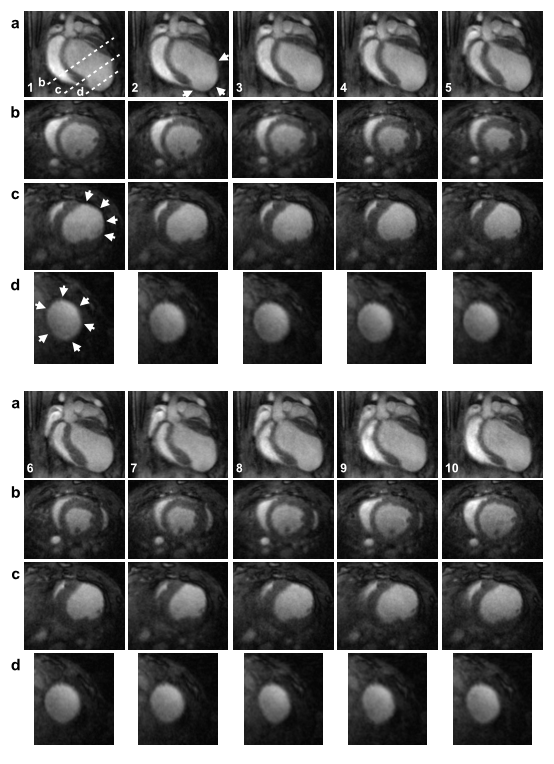
\includegraphics[scale=0.5]{./figure/chap6/Fig9.png}
\caption[Exemple de carte de vitesse \textit{in vivo}]{\label{fig:CarteVitesse}\textbf{Exemple de carte de vitesse \textit{in vivo}.} Images extraites des 10 volumes 3D en orientation coronale obtenues avec la séquence de flux UTE 4D. \textbf{(a)} Image en magnitude. Carte de vitesse obtenues selon la direction X  \textbf{(b)}, selon la diction Y \textbf{(c)}, selon la direction Z \textbf{(d)} et en vitesse absolue \textbf{(e)}.}
\line(1,0){400} \\ 
\end{figure}

\subsection{Quantification préliminaire des vitesses sur un modèle d'hypertension artérielle pulmonaire}

5 souris mâles OB1 ont été imagées (35-40g) durant cette étude, dont 3 d'entre elles ont développé une hypertension artérielle pulmonaire (HTAP) après avoir passé 21 jours dans un caisson hypobare à une pression de 50 kPa.
Les vitesses ont été mesurées dans la crosse aortique et une des artères pulmonaires, les résultats sont présentées dans la figure \ref{fig:CarteVitesse}. On observe que les vitesses maximales mesurées au cours du cycle cardiaque chez les souris HTAP ($v = 30,3 \pm 5,7 m.s^{-1}$) sont plus faibles que chez les souris contrôles ($v = 54,0 \pm 2,8 m.s^{-1}$) en particulier au niveau de l'artère pulmonaire.

Cette diminution de vitesse des flux dans sur les modèles HTAP a déjà été observée dans une précédente étude réalisée sur le rat \cite{Dumas2011effect} avec la stratégie d'angiographie par résonance magnétique dynamique cartésienne présentée dans le chapitre \ref{Chap3}. De plus, cette étude montre aussi la cohérence des données obtenues avec d'autres travaux qui ont étudié la pression sanguine et le débit cardiaque \cite{pozeg2003vivo,hessel2006characterization}.

\begin{figure}[H]
\centering
\line(1,0){400} \\
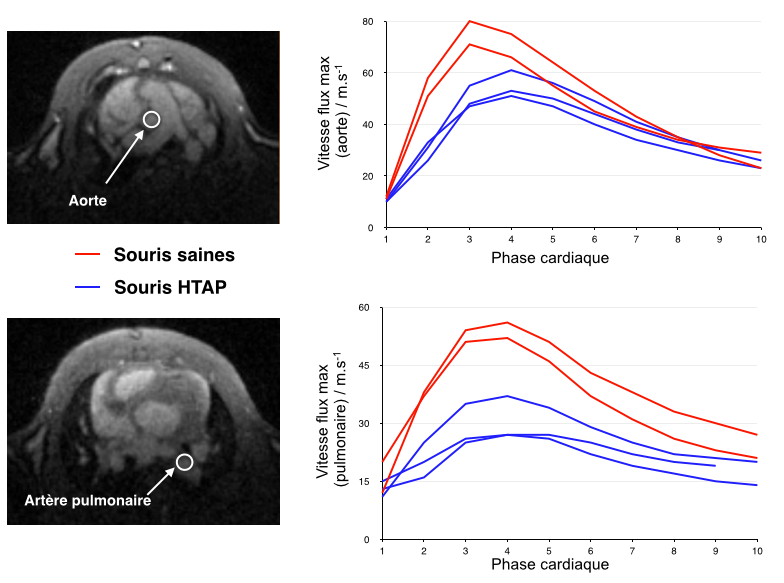
\includegraphics[scale=0.6]{./figure/chap6/Fig10.png}
\caption[Mesure des vitesse chez des souris saine versus HTAP.]{\label{fig:CarteVitesse}\textbf{Mesure des vitesse chez des souris saine versus HTAP.} Schéma présentant les mesures des vitesses maximales effectuées chez 3 souris ayant développé un syndrôme HTAP et 2 souris saines. Les mesures ont été effectuées au niveau de l'aorte (région d'intérêt indiquée sur l'image du haut) et sur une artère pulmonaire (région d'intérêt indiquée sur l'image du bas)}
\line(1,0){400} \\ 
\end{figure}

\section{Discussion}

L'imagerie 4D de flux basée sur le principe du contraste de phase est une méthode arrivée à maturité. Le nombre d'applications cardiovasculaires va en gradissant \cite{Stankovic:2014aa,Garcia:2014aa,Petersson:2015aa}, en particulier grâce aux différentes méthodes permettant de réduire le temps d'acquisition des séquences \cite{Liu:2014aa} ou à la robustesse des méthodes d'analyse développées \cite{Eriksson:2010aa}. Cependant cette stratégie est pour le moment restreinte à l'imagerie chez l'homme. En effet, le peu de travaux publiés chez le petit animal utilise encore des acquisitions 2D résolues dans le temps \cite{Zhao:2009ng}. 

Notre objectif a donc été de développé une méthode robuste en 4D permettant d’obtenir des mesures précises de flux du système cardiovasculaire chez le petit animal. Cette stratégie s’est appuyée sur les résultats obtenus précédemment avec la séquence UTE combinée à l'utilisation d'agent de contraste à base de nanoparticules de fer.

Le rehaussement du signal par injection d’un agent de contraste intravasculaire a deux avantages. Le premier est qu’il permet d’améliorer le rapport signal-sur-bruit des images en magnitude et de réduire le bruit sur les cartes de vitesse. Celui-ci est en effet inversement proportionnel au rapport signal-sur-bruit. Comme montré par Bock et al \cite{Bock:2010aa} l’amélioration du signal permet d’améliorer significativement la visualisation et la quantification des flux sanguins chez l’homme.

Le deuxième avantage est qu’il permet d’obtenir un très bon contraste-sur-bruit entre le sang et les tissus environnants (myocarde, poumons, muscles etc). Ce contraste peut être mis à profit pour facilement segmenter les données de phase à l’aide des données en magnitude. L’analyse des images 4D devient ainsi plus aisée. Même si nous n’avons pas encore utilisé cette avantage, la précision dans le cas de mesure de débit ou de vitesse moyenne a donc de grande chance d’être améliorée avec l’injection d’agents de contraste intravasculaire. 

De plus, en ce qui concerne notre étude, il sera possible grâce au contraste obtenu de réaliser avec précision l’analyse volumétrique des différents paramètres cardiaques (volumes des ventricules durant la systole et diastole, fraction d’ejection, …) sans nécessité de réaliser des acquisitions supplémentaires. Ces analyses devraient montrer des différences significatives entre les deux groupes d’animaux \cite{Miraux:2009rm}. Elles pourront être mises en relation avec les mesures de vitesses obtenues dans les différents vaisseaux. Le modèle d’HTAP pourrait ainsi être entièrement caractérisé \textit{in vivo}.

L’utilisation d’une séquence avec une trajectoire UTE et des gradients bipolaires intenses permet de conserver des temps d’écho inférieurs à 0,6 ms. Cela permet d’une part d’obtenir un signal positif avec des agents de contraste à base de nanoparticules de fer mais aussi de réduire la sensibilité de la séquence aux artefacts de flux. Ceci a été confirmé par l’étude \textit{in vitro} réalisée sur un fantôme de flux dont les mesures de vitesses obtenues avec la séquence UTE montrent une très faible dispersion et sont cohérents avec les vitesses de flux imposées. \textit{In vivo}, aucune disparition de signal, même au niveau de zones turbulentes comme les ventricules cardiaques n’est observée. La mesure de flux devient possible sur l’entièreté du système cardio-pulmonaire de l’animal, ce qui n’avait jamais été montré jusqu’à maintenant.

Dans la littérature, seules deux études font état de l'utilisation d'une méthode 4D de mesure de flux par contraste de phase chez la souris. Janiczek et al \cite{Janiczek:2011qm} utilisent une trajectoire 3D de type empilement de spirales (Stack-Of-Spirals). Cette méthode permet d'atteindre des TE courts (TE = 850 $\mu s$) et dispose ainsi des mêmes propriétés de robustesse vis-à-vis des artefacts de flux dans les zones tortueuses. La résolution spatiale et le temps d'acquisition sont de l'ordre de ceux de nos expériences. Néanmoins, afin d’obtenir un rapport signal-sur-bruit important par effet temps-de-vol, leur champ de vue est limité à l’exploration de la crosse aortique (< à 5,5 mm dans la direction de coupe). Contrairement à nos travaux, il ne leur est pas possible de mesurer simultanément le flux dans d’autres vaisseaux ou dans le coeur.

A notre connaissance Bovenkamp et al \cite{bovenkamp2014velocity} sont les seuls à avoir appliqué une méthode de mesure de flux 4D sur le coeur entier chez la souris. Leur étude est basée sur l'utilisation d'une séquence cartésienne sans injection d'agent de contraste.
Néanmoins, le faible signal sanguin dû à l'absence d'effet temps-de-vol en imagerie 3D ainsi que la diminution du signal  provoquée par des temps d'écho importants de 2,2 ms explique le choix d'utiliser une faible résolution spatiale pour leurs images ($140 \times 200 \times 500 \mu m$) ainsi qu'un nombre d'accumulation de 3 pour obtenir un rapport signal-sur-bruit suffisant. Le temps d’acquisition devient ainsi supérieur à une heure pour des images avec un rapport signal-sur-bruit relativement faible pour le sang.

Il est à noter que les deux méthodes décrites dans la littérature permettent d'atteindre des résolutions temporelles inférieures d'un facteur deux à celle de notre stratégie. Cependant, la méthode d’encodage que nous avons proposée est extrêmement flexible et favorable au sous-échantillonage puisqu’à chaque TR le centre de l’espace de Fourier est encodé. Elle devrait permettre d’augmenter la résolution temporelle des images, mais néanmoins au détriment de la résolution spatiale.

En conclusion, la stratégie développée dans ce chapitre apparaît extrêmement prometteuse. Il a ainsi été montré qu’elle était peu sensible aux déphasages provoqués par les flux turbulents, qu’elle permettait de visualiser les flux dans tout le système cardiovasculaire y compris les cavités cardiaques et qu’enfin, une seule acquisition était nécessaire pour obtenir des informations anatomiques et fonctionnelles.
La résolution spatiale et le rapport signal-sur-bruit des images obtenues sont supérieurs comparé aux autres méthodes décrites dans la littérature pour des champs de vue plus importants et des temps d’acquisition légèrement plus faibles. Cette méthode semble donc idéale en particulier dans le cadre du phénotypage ou d’études de pathologies chez le petit animal dans lesquelles les modifications de vitesses peuvent apparaître comme des modèles d’artérioscléroses ou d’hypertension.

\section{Perspectives}

Un certain nombre de développements restent encore à effectuer, notamment en ce qui concerne le traitement des données. En effet, il est nécessaire de mettre en place un protocole d’analyse des données de flux permettant l’extraction des vitesses moyennes ou maximales dans les vaisseaux ou bien pour la visualisation et la quantification des trajectoires des flux.

De plus, dans le cadre de la réduction du temps d’acquisition total des images ou de l’augmentation de la résolution temporelle, il sera nécessaire d’évaluer précisément l’impact de l’effet du sous-échantillonnage des données sur la mesure des vitesses. Ceci ne pourra être réalisé qu’avec une méthode d’analyse des flux robustes. 

Une collaboration a été mise en place avec l’Université de Northwestern pour le traitement des données. Les résultats présentés ici seront ensuite soumis à publication dans la revue Magnetic Resonance in Medicine.
